\documentclass{beamer}

\usepackage{amsmath}
\usepackage{cancel}
\usepackage{hyperref}
\usepackage{mathtools}
\usepackage{multirow}
\usepackage{tikz, pgfplots}
\pgfplotsset{compat=1.18}

\title{Applying the Klein-Gordon Theory to Gravitation}

\subtitle{Modelling Newtonian gravitation as a classical scalar field theory obeying Klein-Gordon structure}

\author{Siddhartha Bhattacharjee}

\institute
{
1B Mathematical Physics \\
University of Waterloo
}

\date{SASMS, Feb 10, 2023}

\begin{document}

\frame{\titlepage}

\begin{frame}
\frametitle{Table of Contents}
\tableofcontents
\end{frame}

\section{Towards Classical Field Theory}

\begin{frame}
\begin{center}
\Huge \textcolor{blue!50!gray}{Towards Classical Field Theory}
\end{center}
\end{frame}

\begin{frame}
\frametitle{The Inverse Square Law}

\begin{itemize}
\item Gravitational force:
\end{itemize}

$$F_m = - G \frac{M m}{r^2}$$

\begin{itemize}
\item Electrostatic force:
\end{itemize}

$$F_e = \frac{1}{4 \pi \epsilon_0} \frac{Q_e q_e}{r^2}$$

\begin{itemize}
\item Magnetic force:
\end{itemize}

$$F_b = \frac{\mu_0}{4 \pi} \frac{Q_b q_b}{r^2}$$
\end{frame}

\subsection{Formal Analogies Between the Gravitational and Electrostatic Forces}

\begin{frame}
\frametitle{Formal Analogies Between the Gravitational and Electrostatic Forces}

\begin{center}
\begin{tabular}{ |c|c|c|c| } 
\hline
& Gravitation & Static electricity \\
\hline
Newton's second law & $a^i = \underset{- \vec{\nabla} V}{\underbrace{- \partial^i V}}$ & $E^i = \underset{- \vec{\nabla} \phi}{\underbrace{- \partial^i \phi}}$ \\
\hline
Gauss' law & $\underset{\vec{\nabla} \cdot \vec{a}}{\underbrace{\sum \limits_{i=1}^3 \nabla_i a^i}} = - 4 \pi G \rho_m$ & $\underset{\vec{\nabla} \cdot \vec{a}}{\underbrace{\sum \limits_{i=1}^3 \nabla_i E^i}} = \frac{1}{\epsilon_0} \rho_e$ \\
\hline
Poisson's equation & $\underset{\nabla^2 V}{\underbrace{\sum \limits_{i=1}^3 \nabla_i \partial^i V}} = 4 \pi G \rho_m$ & $\underset{\nabla^2 \phi}{\underbrace{\sum \limits_{i=1}^3 \nabla_i \partial^i \phi}} = - \frac{1}{\epsilon_0} \rho_e$ \\  
\hline
\end{tabular}
\end{center}
\end{frame}

\subsection{Classical Mechanics}

\begin{frame}
\frametitle{Lagrangian Mechanics}

\begin{center}
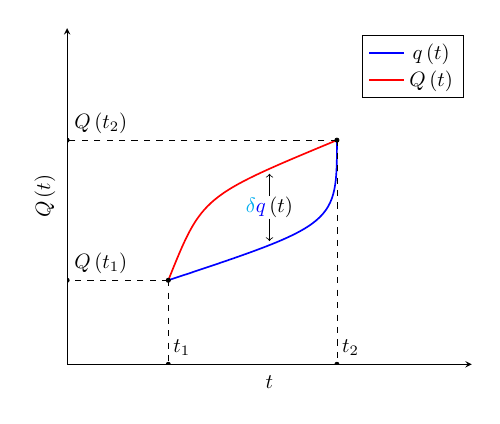
\begin{tikzpicture}[scale=0.75]
\begin{axis}[
    axis lines = left,
    xlabel = $t$,
    ylabel = $Q \left( t \right)$,
    xtick = \empty,
    ytick = \empty,
    xmin=0, xmax=3,
    ymin=0, ymax=3,
]

\draw[thick, blue] (0.75, 0.75) .. controls (2, 1.25) .. (2, 2);
\addlegendimage{thick, color=blue};
\addlegendentry{$q \left( t \right)$};

\draw[thick, red] (0.75, 0.75) .. controls (1, 1.5) .. (2, 2);
\addlegendimage{thick, color=red};
\addlegendentry{$Q \left( t \right)$};

\draw[->] (1.5, 1.5) to (1.5, 1.7);
\draw[->] (1.5, 1.3) to (1.5, 1.1);
\node[] at (1.5, 1.4) {$\textcolor{cyan}{\delta} \textcolor{blue}{q} \left( t \right)$};

\draw[dashed] (0.75, 0.75) -- (0.75, 0);
\draw[dashed] (0.75, 0.75) -- (0, 0.75);
\draw[dashed] (2, 2) -- (2, 0);
\draw[dashed] (2, 2) -- (0, 2);
\node[] at (0.85, 0.15) {$t_1$};
\node[] at (2.1, 0.15) {$t_2$};
\node[] at (0.25, 0.9) {$Q \left( t_1 \right)$};
\node[] at (0.25, 2.15) {$Q \left( t_2 \right)$};

\filldraw[] (0.75, 0.75) circle (1 pt);
\filldraw (2, 2) circle (1 pt);
\filldraw (0.75, 0) circle (1 pt);
\filldraw (0, 0.75) circle (1 pt);
\filldraw (2, 0) circle (1 pt);
\filldraw (0, 2) circle (1 pt);

\end{axis}
\end{tikzpicture}
\end{center}

\begin{itemize}
\item Nature 'selects' the unique on-shell trajectory $\textcolor{blue}{q \left( t \right)}$ given the boundary conditions $\left( t_1, \textcolor{red}{Q \left( t_1 \right)} \right)$ and $\left( t_2, \textcolor{red}{Q \left( t_2 \right)} \right)$ for a system.

\begin{align*}
\underset{\text{Off-shell}}{\underbrace{\textcolor{red}{Q \left( t \right)}}} & = \underset{\text{On-shell}}{\underbrace{\textcolor{blue}{q \left( t \right)}}} + \underset{\text{Variation}}{\underbrace{\textcolor{cyan}{\delta} \textcolor{blue}{q} \left( t \right)}} \\
\textcolor{cyan}{\delta} \textcolor{blue}{q \left( t_1 \right)} & = \textcolor{cyan}{\delta} \textcolor{blue}{q \left( t_2 \right)} = 0
\end{align*}
\end{itemize}
\end{frame}

\begin{frame}
\begin{itemize}
\item Each trajectory $\textcolor{red}{Q \left( t \right)}$ between the endpoints is associated with a corresponding number called the action.

$$\boxed{S \left[ \textcolor{red}{Q \left( t \right)} \right] \left( t_1, t_2 \right) = \int_{t_1}^{t_2} dt \: L \left( \textcolor{red}{Q \left( t \right)}, \textcolor{red}{\dot{Q} \left( t \right)}, t \right)}$$

The integrand $L \left( \textcolor{red}{Q \left( t \right)}, \textcolor{red}{\dot{Q} \left( t \right)}, t \right)$ is known as the Lagrangian of the system being modelled and encodes the dynamics of the system.

\item In general, the action $S$ maps $\textcolor{red}{Q \left( t \right)}$ to a real number determined by the above integral. Therefore, it is a functional, i.e. a higher-order function which takes in infinite values of the form $\left\{ \left( t, \textcolor{red}{Q \left( t \right)} \right) : t \in \mathbb{R} \right\}$ and spits out a real.
\end{itemize}

$$
S : \begin{cases} \mathbb{R}^\mathbb{R} & \to \mathbb{R} \\ \textcolor{red}{Q \left( t \right)} & \mapsto \displaystyle{\int}_{t_1}^{t_2} dt \: L \left( \textcolor{red}{Q \left( t \right)}, \textcolor{red}{\dot{Q} \left( t \right)}, t \right) \end{cases}
$$
\end{frame}

\begin{frame}
\frametitle{Principle of Stationary Action}

\begin{block}{Lagrange's principle of stationary action}
Suppose we vary $\textcolor{blue}{q \left( t \right)}$ about its on-shell evolution as, $\textcolor{blue}{q \left( t \right)} \to \textcolor{blue}{q \left( t \right)} + \textcolor{cyan}{\delta} \textcolor{blue}{q} \left( t \right)$. Then, the variation in the action satisfies,

$$\textcolor{cyan}{\delta} S = \mathcal{O} \left( \textcolor{cyan}{\delta} \textcolor{blue}{q}^2  \right)$$
\end{block}

\begin{corollary}[First-order approximation]
For very small $\delta q \left( t \right)$ i.e.,

\begin{align*}
\forall \: \textcolor{cyan}{\delta} \textcolor{blue}{q} \left( t \right) & = \lim_{\textcolor{cyan}{\epsilon} \to 0} \textcolor{cyan}{\epsilon} \eta \left( t \right) : \eta \left( t_1 \right) = \eta \left( t_2 \right) = 0 : \\
\textcolor{cyan}{\delta} S & = \mathcal{O} \left( \textcolor{cyan}{\cancel{\epsilon^2}} \left( \eta \left( t \right) \right)^2 \right) = 0
\end{align*}
\end{corollary}
\end{frame}

\begin{frame}
\frametitle{Euler-Lagrange Equation}

\begin{lemma}[Fundamental lemma of calculus of variations]
The former is possible if and only if the latter is,

\begin{align*}
\forall \: \textcolor{cyan}{\delta} \textcolor{blue}{q} : \int_{t_1}^{t_2} dt \: \textcolor{cyan}{\delta} \textcolor{blue}{q} \: f \left( \textcolor{blue}{q}, \textcolor{blue}{\dot{q}}, t \right) & = 0 \\
\Longleftrightarrow \forall \: t \in \left( t_1, t_2 \right) : f \left( \textcolor{blue}{q}, \textcolor{blue}{\dot{q}}, t \right) & = 0
\end{align*}
\end{lemma}

\begin{theorem}
An on-shell $\textcolor{blue}{q \left( t \right)}$ obeying the principle of stationary action for a given $L \left( \textcolor{blue}{q}, \textcolor{blue}{\dot{q}}, t \right)$ must also obey the Euler-Lagrange equation of motion:

$$\boxed{\underset{\text{Generalized force}}{\underbrace{\frac{\partial L}{\partial \textcolor{blue}{q}}}} = \underset{\text{Conjugate momentum}}{\frac{d}{dt} \underbrace{\frac{\partial L}{\partial \textcolor{blue}{\dot{q}}}}} = \frac{d \textcolor{blue}{p}}{dt}}$$
\end{theorem}
\end{frame}

\begin{frame}
\begin{block}{Proof.}
\begin{align*}
\textcolor{cyan}{\delta} S & = 0 & \left[ \text{Principle of stationary action} \right] \\
\textcolor{cyan}{\delta} \int_{t_1}^{t_2} dt \: L \left( \textcolor{blue}{q}, \textcolor{blue}{\dot{q}}, t \right) & = 0 \\
\int_{t_1}^{t_2} dt \: \textcolor{cyan}{\delta} L \left( \textcolor{blue}{q}, \textcolor{blue}{\dot{q}}, t \right) & = 0 & \left[ \text{Additivity of variations} \right] \\
\int_{t_1}^{t_2} dt \left[  \textcolor{cyan}{\delta} \textcolor{blue}{q} \frac{\partial L}{\partial \textcolor{blue}{q}} + \textcolor{cyan}{\delta} \textcolor{blue}{\dot{q}} \frac{\partial L}{\partial \textcolor{blue}{\dot{q}}} + \cancel{\textcolor{cyan}{\delta} t} \frac{\partial L}{\partial t} \right] & = 0 & \left[ \text{Chain rule for variations} \right] \\
\int_{t_1}^{t_2} dt \left[  \textcolor{cyan}{\delta} \textcolor{blue}{q} \frac{\partial L}{\partial \textcolor{blue}{q}} + \dot{\left( \textcolor{cyan}{\delta} \textcolor{blue}{{q}}\right)} \frac{\partial L}{\partial \textcolor{blue}{\dot{q}}} \right] & = 0 & \left[ \text{Commutativity of derivatives} \right] \\
\int_{t_1}^{t_2} dt \: \textcolor{cyan}{\delta} \textcolor{blue}{q} \frac{\partial L}{\partial \textcolor{blue}{q}} + \int_{t_1}^{t_2} dt \: \dot{\left( \textcolor{cyan}{\delta} \textcolor{blue}{{q}}\right)} \frac{\partial L}{\partial \textcolor{blue}{\dot{q}}} & = 0
\end{align*}
\end{block}
\end{frame}

\begin{frame}
\begin{block}{Proof.}
\begin{align*}
\int_{t_1}^{t_2} dt \: \textcolor{cyan}{\delta} \textcolor{blue}{q} \frac{\partial L}{\partial \textcolor{blue}{q}} + \frac{\partial L}{\partial \textcolor{blue}{\dot{q}}} \int_{t_1}^{t_2} dt \: \dot{\left( \textcolor{cyan}{\delta} \textcolor{blue}{{q}}\right)} - \int_{t_1}^{t_2} dt \left[ \int dt \: \dot{\left( \textcolor{cyan}{\delta} \textcolor{blue}{{q}}\right)} \right] \frac{d}{dt} \frac{\partial L}{\partial \textcolor{blue}{\dot{q}}} & = 0 \\
\left[ \text{Integration by parts} \right] \\
\int_{t_1}^{t_2} dt \: \textcolor{cyan}{\delta} \textcolor{blue}{q} \frac{\partial L}{\partial \textcolor{blue}{q}} + \frac{\partial L}{\partial \textcolor{blue}{\dot{q}}} \cancel{\left[ \textcolor{cyan}{\delta} \textcolor{blue}{{q}}\right]}_{t_1}^{t_2} - \int_{t_1}^{t_2} dt \: \textcolor{cyan}{\delta} \textcolor{blue}{q} \frac{d}{dt} \frac{\partial L}{\partial \textcolor{blue}{\dot{q}}} & = 0 \\
\left[ \textcolor{cyan}{\delta} \textcolor{blue}{q} \left( t_1 \right) = \textcolor{cyan}{\delta} \textcolor{blue}{q} \left( t_2 \right) \right] \\
\forall \: \textcolor{cyan}{\delta} \textcolor{blue}{q} : \int_{t_1}^{t_2} dt \textcolor{cyan}{\delta} \textcolor{blue}{q} \left( \frac{\partial L}{\partial \textcolor{blue}{q}} - \frac{d}{dt} \frac{\partial L}{\partial \textcolor{blue}{\dot{q}}} \right) & = 0 \\
\Longleftrightarrow \frac{\partial L}{\partial \textcolor{blue}{q}} - \frac{d}{dt} \frac{\partial L}{\partial \textcolor{blue}{\dot{q}}} & = 0 \\
\Longleftrightarrow \frac{\partial L}{\partial \textcolor{blue}{q}} - \frac{d \textcolor{blue}{p}}{dt} & = 0 & \square \\
\left[ \text{Fundamental lemma of the calculus of variations} \right]
\end{align*}
\end{block}
\end{frame}

\begin{frame}
\frametitle{Noether's Theorem}

\begin{theorem}[Noether's first theorem]
If the action $S \left[ \textcolor{blue}{q \left( t \right)} \right]$ remains invariant under perturbations of the following form,

$$\textcolor{blue}{q} \to \textcolor{blue}{q} + \textcolor{cyan}{\delta} \textcolor{blue}{q}$$

then the following quantity is conserved,

\begin{align*}
j & = \textcolor{blue}{p} \: \textcolor{cyan}{\delta} \textcolor{blue}{q} \\
\frac{dj}{dt} & = 0
\end{align*}
\end{theorem}
\end{frame}

\begin{frame}
\begin{block}{Proof.}
\begin{align*}
\textcolor{cyan}{\delta} L & = \frac{\partial L}{\partial \textcolor{blue}{q}} \textcolor{cyan}{\delta} \textcolor{blue}{q} + \frac{\partial L}{\partial \textcolor{blue}{\dot{q}}} \textcolor{cyan}{\delta} \textcolor{blue}{\dot{q}} \\
& = \dot{p} \textcolor{cyan}{\delta} \textcolor{blue}{q} + p \textcolor{cyan}{\delta} \textcolor{blue}{\dot{q}} & \left[ \text{Euler-Lagrange equation} \right] \\
& = \frac{d}{dt} \left( p \textcolor{cyan}{\delta} \textcolor{blue}{q} \right) \\
\text{But} \: \textcolor{cyan}{\delta} L & = 0 \\
\implies \frac{d}{dt} \left( p \textcolor{cyan}{\delta} \textcolor{blue}{q} \right) & = 0 & \square
\end{align*}
\end{block}

\begin{example}
If $S \left[ \textcolor{blue}{q \left( t \right)} \right]$ is symmetric (i.e. conserved) under a small time-independent translation $\textcolor{blue}{q} \to \textcolor{blue}{q} + \textcolor{cyan}{\epsilon}$, we obtain the invariant $j = \textcolor{blue}{p} \textcolor{cyan}{\epsilon}$. Since $\frac{dj}{dt} = 0, \frac{d \textcolor{cyan}{\epsilon}}{dt} = 0$, we get $\frac{d \textcolor{blue}{p}}{dt} = 0$.
\end{example}
\end{frame}

\begin{frame}
\frametitle{Classical Mechanics}

\begin{itemize}
\item The Lagrangian for classical mechanics is of the form,

\begin{align*}
L \left( q, \dot{q}, t \right) & = T \left( \dot{q} \right) - V \left( q \right) \\
& = \frac{1}{2} m \mathit{g} \dot{q}^2 - V \left( q \right) \\
& = \frac{1}{2} mv^2 - V \left( q \right)
\end{align*}

\item The equation of motion obtained by applying the Euler-Lagrange equation to the above Lagrangian is,

$$\frac{d}{dt} \left( m v \right) + \frac{\partial V}{\partial q} = 0$$

This is Newton's second law. If the entire system concerned is symmetric under small translations on $q$, we have $\frac{\partial V}{\partial q} = 0$ implying $\frac{d}{dt} \left( m v \right) = 0$. This is Newton's third law.
\end{itemize}
\end{frame}

\subsection{Classical Field Theory}

\begin{frame}
\frametitle{Classical Field Theory}

\begin{itemize}
\item A classical field is a tensor field on spacetime (which is a pseudo-Riemannian manifold obeying dynamical field equations such as the Einstein field equations).

Therefore, a classical field is some rank $\left( p, q \right)$ tensor $\phi^{\mu_1 \dots \mu_p}_{\phantom{\mu_1 \dots \mu_p} \nu_1 \dots \nu_q} \left( x^\alpha \right)$ at each point $x^\alpha$ in space and time with $\alpha \in \left( 0, 1, 2, 3 \right)$.

\item A classical field obeys the following principles:

\begin{enumerate}
\item Principle of stationary action

\item Local Lorentz invariance

\item Locality

\item Gauge invariance
\end{enumerate}

\item The simplest classical field theory is that of rank $\left( 0, 0 \right)$ tensor fields i.e. scalar fields $\phi \left( x^\alpha \right)$, in a flat spacetime $\mathcal{M}$. We will study such fields in the following slides.
\end{itemize}
\end{frame}

\begin{frame}
\frametitle{Principle of Stationary Action for Classical Fields}

\begin{center}
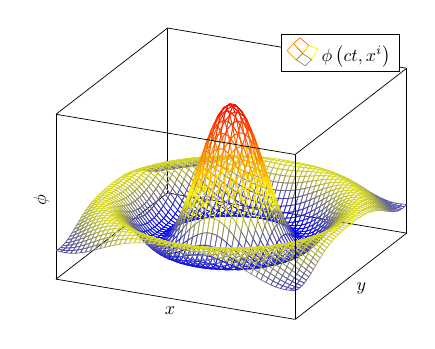
\begin{tikzpicture}[scale=0.65]
\begin{axis}[
xlabel = $x$,
ylabel = $y$,
zlabel = $\phi$,
xtick = \empty,
ytick = \empty,
ztick = \empty,
3d box = complete*,
]
 
\addplot3[
mesh,
samples=50,
domain=-8:8,
]
{sin(deg(sqrt(x^2+y^2)))/sqrt(x^2+y^2)};
\addlegendentry{$\phi \left( ct, x^i \right)$} 

\end{axis}
\end{tikzpicture}
\end{center}

\begin{itemize}
\item To construct the action for a particle, we integrated its Lagrangian between endpoints in time. A field such as $\phi \left( x^\alpha \right)$, however, lives in space and time. Therefore, its action is a \emph{volume} integral of a Lagrangian \emph{density} $\mathcal{L}$, in a 4-dimensional region of spacetime $\Omega \subset \mathcal{M}$,

$$\boxed{S \left[ \phi \left( x^\alpha \right) \right] = \int_\Omega d^4 x \: \mathcal{L} \left( \phi \left( x^\alpha \right), \partial_\mu \phi \left( x^\alpha \right), x^\nu \right)}$$
\end{itemize}
\end{frame}

\begin{frame}
\begin{itemize}
\item The Lagrangian density is so-called as it looks like a Lagrangian (integrable over some time interval $\Omega^{\left( 1 \right)}$) when integrated over a region of space $\Omega^{\left( 3 \right)}$:

\begin{align*}
L \left( \phi \left( x^\alpha \right), \partial_\mu \phi \left( x^\alpha \right), x^\nu \right) & = \int_{\Omega^{\left( 3 \right)}} d^3 x \: \mathcal{L} \left( \phi \left( x^\alpha \right), \partial_\mu \phi \left( x^\alpha \right), x^\nu \right) \\
S \left[ \phi \left( x^\alpha \right) \right] & = \int_\Omega d^4 x \: \mathcal{L} \left( \phi \left( x^\alpha \right), \partial_\mu \phi \left( x^\alpha \right), x^\nu \right) \\
& = \int_{\Omega^{\left( 1 \right)}} c dt \: L \left( \phi \left( x^\alpha \right), \partial_\mu \phi \left( x^\alpha \right), x^\nu \right)
\end{align*}

\item The principle of stationary action for fields states that for small variations $\delta \phi$ of a field $\phi$ in its on-shell configuration, the action remains stationary,

$$\boxed{\delta S = 0}$$
\end{itemize}
\end{frame}

\begin{frame}
\frametitle{Euler-Lagrange Equation for Classical Fields}

\begin{lemma}[Fundamental lemma of multivariable calculus of variations]

\begin{align*}
\forall \: \delta \phi : \int_{\Omega} d^4 x \delta \phi \: f \left( \phi, \partial_\mu \phi, x^\nu \right) & = 0 \\
\Longleftrightarrow \forall \: x^\alpha \in \Omega \backslash \partial \Omega : f \left( \phi, \partial_\mu \phi, x^\nu \right) & = 0
\end{align*}
\end{lemma}

\begin{block}{Einstein summation convention}

Dummy indices, i.e. pairs of upper and lower tensor indices, are implicitly summed over.
\end{block}

\begin{example}
$$A_\mu B^\mu = \sum_{\mu=0}^3 A_\mu B^\mu$$
\end{example}
\end{frame}

\begin{frame}
\begin{Theorem}
A field $\phi$ obeys the principle of stationary action if and only if it also satisfies,

$$\boxed{\frac{\partial \mathcal{L}}{\partial \phi} = \underset{\text{Conjugate momentum tensor}}{\nabla_\mu \underbrace{\frac{\partial \mathcal{L}}{\partial \left( \partial_\mu \phi \right)}}} = \nabla_\mu \pi^\mu}$$
\end{Theorem}

\begin{block}{Proof.}
\begin{align*}
\delta S & = 0 & \left[ \text{Principle of stationary action} \right] \\
\delta \int_\Omega d^4 x \: \mathcal{L} & = 0 \\
\int_\Omega d^4 x \: \delta \mathcal{L} & = 0 & \left[ \text{Additivity of variations} \right]
\end{align*}
\end{block}
\end{frame}

\begin{frame}
\begin{align*}
\int_\Omega d^4 x \left[ \delta \phi \frac{\partial \mathcal{L}}{\partial \phi} + \delta \left( \partial_\mu \phi \right) \underset{\pi^\mu}{\underbrace{\frac{\partial \mathcal{L}}{\partial \left( \partial_\mu \phi \right)}}} + \cancel{\delta x^\mu} \partial_\mu \mathcal{L} \right] & = 0 \\
\left[ \text{Multivariable chain rule for variations} \right] \\
\int_\Omega d^4 x \left[ \delta \phi \frac{\partial \mathcal{L}}{\partial \phi} + \left( \partial_\mu \delta \phi \right) \pi^\mu \right] & = 0 \\
\left[ \text{Commutativity of variations and covariant derivatives} \right] \\
\int_\Omega d^4 x \: \delta \phi \frac{\partial \mathcal{L}}{\partial \phi} + \pi^\mu \underset{\text{Constant surface term}}{\underbrace{\int_\Omega d^4 x \: \partial_\mu \delta \phi}} - \int_\Omega d^4 x \left[ \int d^4 x \: \partial_\mu \delta \phi \right] \nabla_\mu \pi^\mu & = 0 \\
\left[ \text{Volume integration by parts} \right] \\
\end{align*}
\end{frame}

\begin{frame}
Using Stokes' theorem, the constant surface term can be set to $0$. We then find,

\begin{align*}
\int_\Omega d^4 x \: \delta \phi \frac{\partial \mathcal{L}}{\partial \phi} - \int_\Omega d^4 x \: \delta \phi \: \nabla_\mu \pi^\mu & = 0 \\
\int_\Omega d^4 x \: \delta \phi \left( \frac{\partial \mathcal{L}}{\partial \phi} - \nabla_\mu \pi^\mu \right) & = 0 \\
\frac{\partial \mathcal{L}}{\partial \phi} - \nabla_\mu \pi^\mu & = 0 \\
\Longleftrightarrow \frac{\partial \mathcal{L}}{\partial \phi} - \nabla_\mu \frac{\partial \mathcal{L}}{\partial \left( \partial_\mu \phi \right)} & = 0 & \square \\
\left[ \text{Fundamental lemma of multivariable calculus of variations} \right]
\end{align*}
\end{frame}

\begin{frame}
\frametitle{Noether's Theorem for Classical Fields}

\begin{theorem}[Field-theoretic Noether's theorem]

If under a small perturbation $x^\alpha \to x^\alpha + \delta x^\alpha$, the action of a field $\phi$ remains invariant, then the following quantity is conserved i.e. has a vanishing divergence,

\begin{align*}
j^\mu & = \pi^\mu \delta \phi - \mathcal{L} \delta x^\mu \\
\nabla_\mu j^\mu & = 0
\end{align*}
\end{theorem}
\end{frame}

\begin{frame}
\begin{block}{Proof.}
\begin{align*}
\delta \mathcal{L} & = \frac{\partial \mathcal{L}}{\partial \phi} \delta \phi + \frac{\partial \mathcal{L}}{\partial \left( \partial_\mu \phi \right)} \delta \left( \partial_\mu \phi \right) \\
& = \left( \nabla_\mu \pi^\mu \right) \delta \phi + \pi^\mu \partial_\mu \delta \phi & \left[ \text{E-L equation} \right] \\
& = \nabla_\mu \left( \pi^\mu \delta \phi \right) \\
\therefore \left( \nabla_\mu \mathcal{L} \right) \delta x^\mu & = \nabla_\mu \left( \pi^\mu \delta \phi \right) \\
\implies \nabla_\mu \left( \pi^\mu \delta \phi - \mathcal{L} \delta x^\mu \right) & = 0 \\
\Longleftrightarrow \nabla_\mu j^\mu & = 0 & \square
\end{align*}
\end{block}
\end{frame}

\begin{frame}
\frametitle{Energy-momentum Tensor}

\begin{corollary}[Conservation of energy-momentum tensor]

Dividing both sides of the above equation by $\delta x^\nu$, we find an explicit conserved tensor called the energy-momentum tensor,

\begin{align*}
T^\mu_{\phantom{\mu} \nu} & = \pi^\mu \partial_\nu \phi - \delta^\mu_{\phantom{\mu} \nu} \mathcal{L} \\
T^{\mu \nu} & = \underset{\text{Inverse Minkowski metric}}{\underbrace{\eta^{\nu \alpha}} T^\nu_{\phantom{\mu} \alpha}} \\
& = \eta^{\nu \alpha} \left( \pi^\mu \partial_\alpha \phi - \delta^\mu_{\phantom{\mu} \alpha} \mathcal{L} \right) \\
& = \pi^\mu \partial^\nu \phi - \eta^{\mu \nu} \mathcal{L}
\end{align*}

$$\boxed{\nabla_\mu T^\mu_{\phantom{\mu} \nu} = \nabla_\mu T^{\mu \nu} = 0}$$
\end{corollary}
\end{frame}

\begin{frame}
\begin{itemize}
\item The energy-momentum tensor $T^{\mu \nu}$ physically represents the flux of $\pi^\mu$ through the surface form $\bigwedge \limits_{\alpha \neq \nu} \text{d} x^\alpha$. This corresponds to the flow of the field's energy($\mu = 0$)/momentum($\mu = 1, 2, 3$) along $x^\nu$.

\item But if we have flow of $\pi^\mu$ in the $x^\nu$ direction, then it implies an energy/momentum in the $x^\nu$ direction. The world line correpsonding to this flow must intersect with the former through a hypersurface of simulteinity, giving rise to equal $T^{\nu \mu}$. 

\item Thus, the energy-momentum tensor, being a geometric object with the mentioned physical meaning (motivated by particle and continuum dynamics), turns out to be symmetric,

$$\boxed{T^{\mu \nu} = T^{\nu \mu}}$$
\end{itemize}
\end{frame}

\section{Klein-Gordon Theory}

\begin{frame}
\begin{center}
\Huge \textcolor{blue!50!gray}{Klein-Gordon Theory}
\end{center}
\end{frame}

\subsection{Klein-Gordon Lagrangian}

\begin{frame}
\frametitle{Klein-Gordon Lagrangian}

\begin{itemize}
\item The classical-field theoretic construction of Klein-Gordon theory begins by asking which Lagrangian yields a symmetric energy-momentum tensor. Such a theory, by virtue of respecting the physical meaning of the energy-momentum tensor, successfully describes many 'physically valid' systems.

\item It turns out that the Klein-Gordon theory is deeply rooted in nature. In quantum mechanics, it is the theory for spin-0 particles. In quantum electrodynamics, the Klein-Gordon theory can be used to construct that of Dirac spinor fields, which describe all massive spin-1/2 particles such as electrons.
\end{itemize}
\end{frame}

\begin{frame}
\begin{itemize}
\item Recall the energy-momentum tensor for a scalar field $\phi$ and its symmetry,

\begin{align*}
T^{\mu \nu} & = \pi^\mu \partial^\nu \phi - \eta^{\mu \nu} \mathcal{L} \\
T^{\mu \nu} & = T^{\nu \mu}
\end{align*}

where $\displaystyle{\pi^\mu = \frac{\partial \mathcal{L}}{\partial \left( \partial_\mu \phi \right)}}$. Thus,

\begin{align*}
\pi^\mu \partial^\nu \phi - \cancel{\eta^{\mu \nu} \mathcal{L}} & = \pi^\nu \partial^\mu \phi - \cancel{\eta^{\nu \mu} \mathcal{L}} & \left[ \eta^{\mu \nu} = \eta^{\nu \mu} \right] \\
\pi^\mu \partial^\nu \phi & = \pi^\nu \partial^\mu \phi
\end{align*}

\item The above is true in the most general case when $\pi^\mu$ is equal to $\partial^\mu \phi$, allowing us to exchange the product of conjugate momentum $\pi^\mu$ and generalized velocity $\partial^\nu \phi$ as above (by commutativity of component multiplication). 
\end{itemize}
\end{frame}

\begin{frame}
Therefore, we have,

\begin{align*}
\pi^\mu & = \partial^\mu \phi \\
\implies \frac{\partial \mathcal{L}}{\partial \left( \partial_\mu \phi \right)} & = \partial^\mu \phi
\end{align*}

'Integrating' over $\partial_\mu \phi$, we find that the Lagrangian is constrained to be of the form,

$$\boxed{\mathcal{L} = \frac{1}{2} \partial_\mu \phi \partial^\mu \phi - V \left( \phi \right)}$$

\begin{itemize}
\item This is the Klein-Gordon Lagrangian $\mathcal{L}_{KG}$. Notice that it is analogous to the Lagrangian for classical mechanics, if we interpret $\frac{1}{2} \partial_\mu \phi \partial^\mu \phi$ as a kinetic term $T \left( \partial_\mu \phi \right)$ and $V \left( \phi \right)$ as a potential term.
\end{itemize}
\end{frame}

\begin{frame}
Indeed,

\begin{align*}
\pi^\mu & = \frac{\partial \mathcal{L}}{\partial \left( \partial_\mu \phi \right)} \\
& = \frac{\partial}{\partial \left( \partial_\mu \phi \right)} \left[ \frac{1}{2} \partial_\alpha \phi \partial^\alpha \phi - V \left( \phi \right) \right] \\
& = \frac{1}{2} \frac{\partial}{\partial \left( \partial_\mu \phi \right)} \left[ \partial_\alpha \phi \partial^\alpha \phi \right] \\
& = \partial^\alpha \phi \frac{\partial}{\partial \left( \partial_\mu \phi \right)} \partial_\alpha \phi \\
& = \partial^\alpha \phi \delta^\mu_{\phantom{\mu} \alpha} \\
& = \partial^\mu \phi
\end{align*}
\end{frame}

\subsection{Klein-Gordon Equation}

\begin{frame}
\frametitle{Klein-Gordon Equation}

\begin{itemize}
\item Let us find the equation of motion for a Klein-Gordon field by plugging its conjugate momentum into the Euler-Lagrange equation:

$$\nabla_\mu \pi^\mu - \frac{\partial \mathcal{L}}{\partial \phi} = 0$$

$$\implies \boxed{\nabla_\mu \partial^\mu \phi + \frac{\partial V}{\partial \phi} = 0}$$

$$\Longleftrightarrow \square \phi + \frac{\partial V}{\partial \phi} = 0$$

\item This is the celebrated Klein-Gordon equation [for a scalar field in a potential]. In the absence of a potential, we obtain the wave equation $\square \phi = 0$.
\end{itemize}
\end{frame}

\begin{frame}
\begin{itemize}
\item For small oscillations of $\phi$ about local minima of the potential $V \left( \phi \right)$, only differences in $\phi$ physically matter. In the series expansion for $\frac{\partial V}{\partial \phi}$, we can set a vanishing first power term. Hence, in the series for $V \left( \phi \right)$, the first power term for $\phi$ vanishes, and so do cubic and higher terms,

$$V \left( \phi \right) = \frac{1}{2} m^2 \phi^2$$

\item Plugging the above potential into the Klein-Gordon equation, we get the Klein-Gordon equation for a scalar field in a potential whose effects locally vanish:

$$\boxed{\nabla_\mu \partial^\mu \phi + m^2 \phi = 0}$$

\item This is analogous to Hooke's law for harmonic oscillators, with mass assuming the role of the 'spring constant'. That's no coincidence -- solutions to the above equation \emph{are} systems of infinite harmonic oscillators at each point in spacetime!
\end{itemize}
\end{frame}

\subsection{Gauge Invariance}
\begin{frame}
\frametitle{Gauge Invariance}

\begin{itemize}
\item Classical fields admit the structure of gauge invariance -- wherein different definitions of the field represent the same physical situation. This happens when the field can encode more information than the physical system being represented.
\end{itemize}

\begin{example}
In electromagnetism, it is possible to add an arbitrary 4-gradient $\partial^\mu s$ to the electromagnetic 4-potential field $A^\mu$, but get the same electromagnetic tensor, which encodes the physics,

\begin{align*}
A^\mu & \to A^\mu + \partial^\mu s & \left[ \text{Gauge transformation} \right] \\
F^{\mu \nu} & = \partial^\mu A^\nu - \partial^\nu A^\mu \\
\therefore F^{\mu \nu} & \to \partial^\mu \left( A^\nu + \partial^\nu s \right) - \partial^\nu \left( A^\mu + \partial^\mu s \right) \\
& = \partial^\mu A^\nu + \cancel{\partial^\mu \partial^\nu s} - \partial^\nu A^\mu - \cancel{\partial^\nu \partial^\mu s} \\
& = F^{\mu \nu}
\end{align*}
\end{example}
\end{frame}

\begin{frame}
\begin{itemize}
\item In general, we want physics to remain the same under a gauge transformation $\phi \to \widetilde{\phi}$ where this transformation belongs to the symmetry group of the gauge theory in question.

This makes us expect that the Euler-Lagrange equation should stay the same under such a transformation -- except it does not! 

This is fixed by allowing gauge structure and modifying the Euler-Lagrange equation by replacing usual covariant derivatives with gauge covariant derivatives (= covariant derivatives + gauge connection term),

\begin{align*}
\partial_\mu \phi & \to D_\mu \phi = \underset{\text{Gauge connection coefficient}}{\partial_\mu \phi - \phi \underbrace{\frac{\partial \phi}{\partial \widetilde{\phi}} \partial_\mu \frac{\partial \widetilde{\phi}}{\phi}}} \\
\pi^\mu & \to \widetilde{\pi}^\mu = \underset{\text{Inverse gauge Jacobian}}{\underbrace{\frac{\partial \phi}{\partial \widetilde{\phi}}} \pi^\mu}
\end{align*}
\end{itemize}
\end{frame}

\begin{frame}
\begin{itemize}
\item Furthermore, if we have multiple similar scalar fields, they start behaving like abstract indexed quantities i.e. abstract tensors.

Since by definition the theory of a real-valued classical field is equivalent to the theory of a single-index classical field theory, we can, for instance, make the correspondances,

\begin{align*}
\phi^{2n} & \leftrightarrow \left( \phi_a \phi^a \right)^n \\
\phi^{2n+1} & \leftrightarrow \left( \phi_a \phi^a \right)^n \phi_b
\end{align*}

\item In the theory of indexed classical fields, the potential must act on a gauge scalar, and the simplest gauge scalar which only depends on the indexed fields $\phi_a$ is $\phi_a \phi^a$. Thus,

$$V = V \left( \phi_a \phi^a \right)$$

In the real-valued classical field theory, this corresponds to asserting,

$$V = V \left( \phi^2 \right)$$
\end{itemize}
\end{frame}

\begin{frame}
\begin{itemize}
\item Therefore, in a series expansion of the potential, odd powers vanish,

$$V \left( \phi^2 \right) = \underset{\text{Coupling constants}}{\sum_{n=1}^\infty \frac{1}{n!} \underbrace{g_n} \phi^{2n}}$$

\item Since we know that in Klein-Gordon theory, $V \left( \phi \right) = \frac{1}{2} m^2 \phi^2 + \mathcal{O} \left( \phi^3 \right)$, in the above, we set $g_1 = \frac{1}{2} m^2 \phi^2$ and write the potential as,

$$V \left( \phi \right) = \frac{1}{2} m^2 \phi^2 + \sum_{n=2}^\infty \frac{g_n}{n!} \phi^{2n}$$
\end{itemize}
\end{frame}

\begin{frame}
\begin{itemize}
\item Thus, the full Klein-Gordon Lagrangian resembles

$$\boxed{\mathcal{L} = \frac{1}{2} \partial_\mu \phi \partial^\mu \phi - \frac{1}{2} m^2 \phi^2 + \sum_{n=2}^\infty \frac{g_n}{n!} \phi^{2n}}$$

\item From the above, the full Klein-Gordon equation resembles,

$$\boxed{\nabla_\mu \partial^\mu \phi + m^2 \phi - 2 \sum_{n=1}^\infty \frac{g_{n+1}}{n!} \phi^{2n+1} = 0}$$

This completes our Klein-Gordon analysis.
\end{itemize}
\end{frame}

\section{Newtonian Gravitation}

\begin{frame}
\begin{center}
\Huge \textcolor{blue!50!gray}{Newtonian Gravitation}
\end{center}
\end{frame}

\subsection{As a Classical Field Theory}

\begin{frame}
\frametitle{As a Classical Field Theory}

\begin{itemize}
\item Newtonian gravitation has two aspects:
\begin{enumerate}
\item How matter, encoded in the mass density field $\rho$, affects the gravitational potential field $\phi$.

\item How the gravitational potential field $\phi$ causes matter to move and hence change the matter density field $\rho$.
\end{enumerate}

Field theory concerns itself with the latter aspect.

\item Unfortunately, Newtonian gravitation is not a classical field theory, as it does not obey local Lorentz invariance and locality. Fixing this requires Einstein's general theory of relativity, where the gravitational field is not a separate tensor field living in spacetime but the metric tensor itself, capturing the geometry of spacetime.
\end{itemize}
\end{frame}

\begin{frame}
\begin{itemize}
\item Fortunately, Newtonian gravitation is \emph{almost} a classical field theory, as it still obeys the principle of stationary action, global Galilean invariance and gauge invariance.

\item The gauge structure of the gravitational potential field $\phi$ is affine, i.e. $\phi \to \phi + s$ where $s$ is a constant, does not change physics, encoded in the gravitational field $g^i = - \partial^i \phi$.

\item As we shall see, the gravitational potential field $\phi$ obeys the principle of stationary action, as its equation of motion, Poisson's equation, can be written as an Euler-Lagrange equation. In fact, it is an example of the Klein-Gordon equation in $D=3$ dimensions!
\end{itemize}
\end{frame}

\subsection{Non-relativistic Klein-Gordon Theory in $D=3$}

\begin{frame}
\frametitle{Non-relativistic Klein-Gordon Theory in $D=3$}

\begin{itemize}
\item The Klein-Gordon theory not only applies in $D=4$ dimensions with special/general relativity, but also $D=3$ dimensions with Galilean relativity! 

This is because the way classical fields are constructed in $D=3$ is analogous to that in $D=4$, except we replace local Lorentz invariance + locality with global Galilean invariance. Furthermore, we replace the Minkowski metric for $D=1+3$ spacetime with the Euclidean metric for $D=3$ space.

\item Except the above, much of the mathematical machinery for fields remains the same in the non-relativistic $D=3$ case, for example -- tensor fields, principle of stationary action, Euler-Lagrange equation, Noether's theorem, energy-momentum tensor and its conservation, etc. 
\end{itemize}
\end{frame}

\subsection{Constructing the Lagrangian}

\begin{frame}
\frametitle{Constructing the Lagrangian}

\begin{itemize}
\item Recall Poisson's equation for the gravitational potential field $\phi$,

$$\nabla_i \partial^i \phi + 4 \pi G \rho = 0$$

In comparison, here's the Klein-Gordon equation in a potential:

$$\nabla_i \partial^i \phi + \frac{\partial V}{\partial \phi} = 0$$

\item Clearly, Poisson's equation can be written as a Klein-Gordon equation by setting $\displaystyle{\frac{\partial V}{\partial \phi} = 4 \pi G \rho}$. The simplest solution for such a $V \left( \phi \right)$ is,

$$V \left( \phi \right) = 4 \pi G \rho \phi$$
\end{itemize}
\end{frame}

\begin{frame}
Thus, the Lagrangian for Newtonian gravitation is,

$$\boxed{\mathcal{L} = \frac{1}{2} \partial_i \phi \partial^i \phi - 4 \pi G \rho \phi}$$
\begin{itemize}
\item A gauge structure inherent to any classical field theory is linearity. I.e., linear transformations of the Lagrangian $\mathcal{L} \to \alpha \mathcal{L} + \beta$ ($\alpha, \beta$ are constants) do not change the corresponding Euler-Lagrange equation.

\item By dividing the obtained Lagrangian by $4 \pi G$, we get an equally valid Lagrangian, which is more commonly used in the physics and mathematics literature,

$$\boxed{\mathcal{L} = \underset{\vec{\nabla} \phi \cdot \vec{\nabla} \phi}{\frac{1}{8 \pi G} \underbrace{\partial_i \phi \partial^i \phi}} - \rho \phi}$$
\end{itemize}
\end{frame}

\subsection{Mass Density Field as a Classical Field}

\begin{frame}
\frametitle{Mass Density Field as a Classical Field}

\begin{itemize}
\item Notice that if we vary the Lagrangian we constructed with respect to the mass density field, we get the [nonsensical] equation:

$$\phi = 0$$

\item Classical field theory deals with this problem by adding a new term $\mathcal{L}_\mathcal{M}$ to the Lagrangian, representing the unspecified theory of matter.

$$\boxed{\mathcal{L} = \frac{1}{8 \pi G} \partial_i \phi \partial^i \phi - \rho \phi + \mathcal{L}_\mathcal{M}}$$

Additionally, we want $\displaystyle{\frac{\delta \mathcal{L}_\mathcal{M}}{\delta \phi} = \rho}$. Such a matter field Lagrangian would respect both Newtonian gravitation and the matter field theory.
\end{itemize}
\end{frame}

\section{References}

\begin{frame}
\frametitle{References}

\begin{enumerate}
\item \textbf{Classical Mechanics:The Theoretical Minimum} by Leonard Susskind

\item \textbf{From Special Relativity to Feynman Diagrams} by Riccardo D'Auria, Mario Trigiante

\item \textbf{The Lagrangian of Newtonian gravity} (\href{https://www.vttoth.com/CMS/physics-notes/269-the-lagrangian-of-newtonian-gravity}{\textcolor{blue}{https://www.vttoth.com/CMS/physics-notes/269-the-lagrangian-of-newtonian-gravity}}) by Viktor T. Toth
\end{enumerate}
\end{frame}

\section{Final Notes}

\begin{frame}
\frametitle{Final Notes}

\begin{itemize}
\item Big thank you to Pure Math Club for hosting this exciting event and to everyone attending this talk!

\item More on this presentation can be found on my blog in the classical field theory section (\href{https://booodaness.github.io/tempus-spatium/categories/classical-field-theory/}{\textcolor{blue}{https://booodaness.github.io/tempus-spatium/categories/classical-field-theory/}}).

\item Source code, pdf for this presentation available at: \href{https://github.com/Booodaness/scientific-documents/tree/master/applying_klein_gordon_theory_gravitation}{\textcolor{blue}{https://github.com/Booodaness/scientific-documents}}

\item Feel free to contact me on Discord at Booodaness\#1464 if you have any questions!
\end{itemize}
\end{frame}

\begin{frame}
\begin{center}
\Huge \textcolor{blue!50!gray}{THANK YOU}
\end{center}
\end{frame}

\end{document}